
\documentclass{amsart}

\usepackage{graphicx}
%\usepackage[altbullet]{lucidabr}
%two lines below change font (font intalled manually (i.e. uploaded))
%\usepackage{fontspec}
%\setmainfont[Ligatures=TeX]{LucidaBrightRegular.ttf}
%\usepackage{kpfonts}    % for nice fonts
% option [light] for more aery documents
\usepackage{color}  %for color of references
\usepackage[dvipsnames]{xcolor} %for color of references
\usepackage{caption}
\usepackage{fancyhdr}
\usepackage[pagebackref,colorlinks, citecolor=BlueViolet,urlcolor=BlueViolet]{hyperref}
\hypersetup{colorlinks = BlueViolet, allcolors = BlueViolet}
\usepackage[nameinlink,noabbrev]{cleveref} 
\usepackage{natbib}
\usepackage{multicol}
\usepackage{multirow}
%\usepackage{lscape}
\usepackage{pdflscape}
\usepackage{amssymb}
\usepackage{geometry}
\usepackage{longtable}
\usepackage{colortbl}
\usepackage{dsfont}
\usepackage{bm}
\usepackage{mathtools}
\usepackage{pgf}
\usepackage{tikz}
\usepackage{soul}
\usepackage{tikz}
\usepackage{tikz,fullpage}
\usepackage{pgf}
\usepackage{tikz}
\usepackage{bbm} %for the indicator function
\usetikzlibrary{shapes.geometric, arrows} %to create flow charts
\usepackage{bold-extra} %for bold small caps in the title
\usepackage{dirtree} % to create lists as tree

%\renewcommand{\familydefault}{\sfdefault} %for the sans serif font

%AMS original setup for mathematical elements
\newtheorem{theorem}{Theorem}[section]
\newtheorem{lemma}[theorem]{Lemma}
\theoremstyle{definition}
\newtheorem{definition}[theorem]{Definition}
\newtheorem{example}[theorem]{Example}
\newtheorem{xca}[theorem]{Exercise}
\theoremstyle{remark}
\newtheorem{remark}[theorem]{Remark}
\numberwithin{equation}{section}

%    Absolute value notation
\newcommand{\abs}[1]{\lvert#1\rvert}

%    Blank box placeholder for figures (to avoid requiring any
%    particular graphics capabilities for printing this document).
\newcommand{\blankbox}[2]{%
  \parbox{\columnwidth}{\centering
%    Set fboxsep to 0 so that the actual size of the box will match the
%    given measurements more closely.
    \setlength{\fboxsep}{0pt}%
    \fbox{\raisebox{0pt}[#2]{\hspace{#1}}}%
  }%
}

%Tikz setup for a flow chart
\tikzstyle{modelblock} = [rectangle, rounded corners, minimum width=3cm, minimum height=1cm,text centered, draw=black, fill=white, text ragged]

\tikzstyle{arrow} = [thick,->,>=stealth]

\begin{document}

\title{EC534 - Referee Report}

%    Information for first author
\author{Arnaud Dy\`evre}
%\address{}
%\curraddr{}
%\email{a.dyevre@lse.ac.uk}
%\thanks{}

%    Information for second author
%\author{}
%\address{}
%\email{}
%\thanks{}

%    General info
%\subjclass[2000]{}

%\date{\today. First created October 19, 2019}

%\dedicatory{}
%\keywords{}

%\begin{abstract}

%\end{abstract}

\maketitle

\begin{center}
Student number: 201324680
\end{center}


\vspace{12pt}

I am refereeing ``The rise of Market Power and Macroeconomic implications'' (November 2019 version) by Jan De Loecker, Jan Eeckhout and Gabriel Unger. The paper is forthcoming in the \textit{Quarterly Journal of Economics}.

%% The correct journal style for \specialsection is all uppercase; a known bug
%% in amsart.cls prevents this, so input must be uppercase until it is fixed.
%\specialsection*{This is a Special Section Head}
%\specialsection*{THIS IS A SPECIAL SECTION HEAD}
%This is an example of a special section head%
%%%%%%%%%%%%%%%%%%%%%%%%%%%%%%%%%%%%%%%%%%%%%%%%%%%%%%%%%%%%%%%%%%%%%%%%
%\footnote{Here is an example of a footnote. Notice that this footnote text is running on so that it can stand as an example of how a footnote with separate paragraphs should be written.
%\par
%And here is the beginning of the second paragraph.}%
%%%%%%%%%%%%%%%%%%%%%%%%%%%%%%%%%%%%%%%%%%%%%%%%%%%%%%%%%%%%%%%%%%%%%%%%
\newpage 

\section{Method}

\begin{itemize}
    \item Go through paper
    \item Go through James Traina's paper
    \item Read Basu (2019)
    \item Go through the note accompanying the paper on Jan de Loecker's website
    \item Go through the JEL papers
\end{itemize}

\section{Summary of the paper}

The paper is an ambitious empirical exercise attempting to document the rise in market power in the US. It uses a novel and microfounded estimation strategy to show that aggregate markups were stable at around a fifth of marginal cost from 1955 to 1980, but they increased to three fifth of marginal cost over 1980-2016. The overall rise in markups is driven by a combination o two effects: the upper tail of the markup distribution has fattened, and high markup firms have captured a larger share of sales. These effects account for 1/3 and 2/3 of the aggregate increase, respectively.\\

The paper uses data on publicly listed firms and on the universe of firms observed in the US Manufacturing, retail and Wholesale Censuses to support this thesis.\\

The paper addresses several criticism related to what the increase in aggregate markups may capture, beyond market power such as a rise in fixed costs, 

It then relates the rise in markups to macroeconomic trends such as the fall in the labour and capital shares, the decline in business dynamism and the decline in labour reallocation.\\

Its main contributions are to (i) , (ii) and (iii).

\section{Summary of the method}

The Industrial Organisation literature has relied on a two-step method--the ``demand approach''--to empirically estimate markups: first, estimate consumer demand, then model how firm compete, and finally combine these insights to estimate how far above marginal costs can prices. This approach is demanding in terms of data, and does not scale well to study larger macroeconomic questions.\\

The authors rely on a method pioneered by \cite{hall1988relation} and refined by \cite{de2012markups}. It consists in backing out markups from the \hl{difference} in the share of a variable input expenditure in total revenue and the output elasticity of this input. The intuition is \hl{...}. The input elasticity is obtained by assuming that the firm minimise costs.\\

there are three approaches to estimating markups:
\begin{itemize}
    \item \textbf{Relying on observed profit margins}. This is straightforward to implement but requires to equate marginal and average costs.
    \item \textbf{The demand approach from IO}.
    \item \textbf{The production approach}. This method only requires the specification of a production function.
\end{itemize}

To compute markups, researchers need to get an estimate of marginal costs. When using the production approach, this is made possible by stating the problem of the firm as a cost-minimisation one. The marginal cost thus naturally appears as the Lagrange multiplier in the cost-minimisation problem. Manipulating the first order condition of the firm allows researchers to express markups as a function of the revenue share of variable inputs and the output elasticity of variable input: $$\mu_{i t}=\epsilon_{i t}^v \frac{P_{i t} Q_{i t}}{P_{i t}^{V} V_{i t}}$$

A crucial component of this formula is thus the output elasticity $\epsilon_{i t}^v$. These elasticities are sector and time-specific. In this paper, they are estimated using a variant of the technique introduced by \cite{olley1996dynamics} to estimate production functions without imposing the assumption of constant return to scale. \\

\subsection*{Comparison with other methods} The method is relatively new, and the cost-minimisation assumption is not entirely standard. Most importantly, if a firm is minimising costs taking input prices as given, this implicitly assumes that firms do not have any wage-setting power. Recent evidence from the US economy show that this assumption may not be totally innocuous \citep{council2016labor}.\\

\subsection*{Assumption of fixed marginal cost for all inputs} \cite{de2019rise} assume that marginal costs are constant across variable inputs. As marginal cost must be the same along each margin, it enables them to use all expenditures on inputs, including labour and intermediate materials, to calculate output elasticities. 

\subsubsection{Aggregation} A contentious part of the paper pertains to how firm-level markups are being aggregated. they calculate aggregate markups as

$$ \mu_{t}=\sum_{i} m_{i t} \mu_{i t} $$ 

where $m_{it}$ is the weight of firm $i$ at $t$. The authors use the sales share of firms as weights. But they show that if input weights are used instead, the rise of markup still holds, but the rise is less pronounced. This result is consistent with the theory: if market power increases, quantity sold and inputs used decrease, but total sales increase through higher prices. Thus using input shares understate the magnitude of markups.\\

\subsection*{Sumary of the robustness checks} Show formula with all changes done by the authors (PF1, PF2, etc...) (see section 4).

\section{Relevance}

\subsection*{Generating economy-wide measures of aggregate markups} The main strength of the paper is to estimate an average markup for the entire US economy. IO scholars had estimated sector- or firm-specific markups before, but overall aggregate markup measures based on firm-level data has been a very recent endeavour.\\

A related strength is the wide time-coverage of the markup measure.\\

\subsection*{Explaining several important secular trends} The paper's relevance cannot be understated. By the authors' account, the rise of markups can explain the fall in labour income, the decline in low-skill wages, the decline in labour force participation, the decline in geographical and inter-firm mobility, and the slowdown in productivity growth. Irrespective of the solidity of the empirical evidence, a single unified explanation for all these phenomena is worthy of exploration. \\

Large, high-markup firms tend to have lower labour shares. This follows mechanically from the firm's optimisation problem that high markups lead to lower expenditure on inputs like labour. Combining this observation with their increased weight in the US economy in terms of sales can allow us to make sense of the secular decline in the labour share. This echoes the findings of \cite{autor2019fall} and \cite{kehrig2017growing}. The authors argue that increased market power is the cause behind the rise of markups and the diminution of the labour share of income.\\

The only issue with this argument is that the timing of their rise in markups does not correspond to that of the fall in the labour share. The labour share drops ralatively sharply in the 2000s but is rather stable before, yet their markup measure increases from the 1980s onward.\\

The paper remains silent about the causes of the rise in market power (technology? change in market structure due to the decline in antitrust enforcement).

\subsection*{Explaining the great moderation} The rise of markups documentaed by the authors could explain the apparent stagnation in American productivity growth since the 1970s. A firm with higher market power can charge higher prices and sell lower quantities, moving up the demand curve. This leads measured GDP to be lower. Hence GDP growth will be constantly lower is markups are steadily increasing.\\

\section{Main findings}



\section{Major comments}

The paper opens itself to two types of criticisms: methodological and theoretical. The methodological concerns are about aggregation and how the share of inputs is calculated.

\subsection*{Composition of the \textit{Compustat} sample} The authors document a positive relationship between markups and firm size within industries. But this source of changes in markups is not presented in the paper. While within firm variation in markups is shown, tyhe authors do not explain if the overall composition of the \textit{Compustat} sample changes over time.\\

\subsection*{Important contribution in the measurement of firm-level markups} The Herfindalh-Hirschman Index (HHI) is inadequate to study markups over time and space as it depends on the definition of a market. \cite{de2019rise} \\

\subsection*{Precision of the measure of markups} One suspects that these measures of markup are very volatile, as seen from the decomposition of aggregate markups

\subsection*{Use of share of sales as weights} This assumption seems discutable. The authors defend this assumption for the three following reasons: as reallocation of sales toward high-markup firms seems to be the driving force behind rising aggregate market power using input shares as weights would miss this trend, profits rates are aggregated with sales shares, and revenue weighting is used in the calculation of macroeconomic indicators such as GDP. These reasons are not entirely convincing. \\

One graph that did not survive in the latest version of the paper shows how important the choice of weights is when aggregating markups from the firm level to an economy-wide average. In the 2017 NBER working paper version, the authors find that the sales share-weighted average of markups is actually lower than the unweighted average. I have reported the series in \ref{fig:unweighted} below. This is counter-intuitive as one would expect the weighted average to be larger than the unweighted one if high markup firms are also those with the largest sales share. This would be consistent with the theoretical prediction of a model of oligopolistic Cournot competition, and with empirical findings from recent papers on the superstar firm \cite{autor2019fall}.

\begin{figure}[h!]
    \centering
    \begin{tabular}{c}
        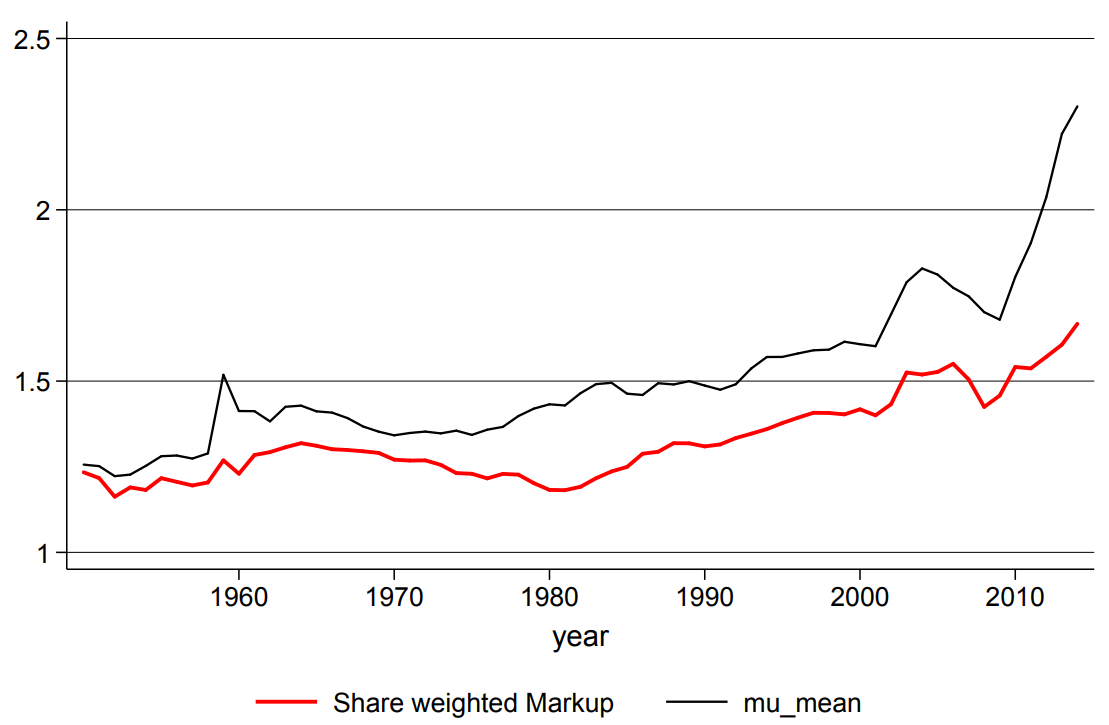
\includegraphics[width=0.8 \textwidth]{unweighted_markups.PNG}
    \end{tabular}
    \centering
    \caption{Unweighted versus weighted markups \\ Figure 2(a) from \cite{deloecker2017rise}}
    \label{fig:unweighted}
\end{figure}

One way to reconcile this finding is to assume that firms with really high markups are in smaller sectors in terms of GDP, and that the difference in market shares in the sector with the highest markup spread is not large. Consider the following simple example: there are two firms in manufacturing, and two firms in farming, the farming firms charge markups of 2 and 1.1, and they represent 11 and 9\% of all sales in the economy respectively. In manufacturing, the biggest firm charges markups of 1.4 and the smallest 1.04, they weight 60 and 20\%. The unweighted average markup is 1.385, the weighted one is 1.403. In sum, the heterogeneity of firms distributions across sectors is what is driving the result. With this observation, we have two options: either conclude that the markups measured by De Loecker and co-authors capture something different from market power, or question the merits of aggregation of such different sectors.\footnote{Another possibility is that small firms charge higher markups, but this would be inconsistent with the aforementioned evidence on superstar firms.}\\

But the authors actually report in the appendix that markups are \textbf{negatively} correlated with size of sales, employment and cost of goods sold. This is a direct contradiction of the superstar firm effect. A closer look at the selection of firm markups reveal that Apple, AT\&T and Microsoft all experienced a decrease in markups. In the NBER working paper version of the paper, they document that markups are negatively correlated with size across industries, but positively correlated with size within. This highlights again the importance of sector heterogeneity. This seems to be an important characterisation of their finding and I believe it would have deserved more discussion in the body of the paper. \\

\subsection*{Comparison with the evolution of industry-level markups}. A welcome addition to the most recent version of the paper consists of the comparison of the DLEU results with those of \cite{hall2018new}. The reason why industry-level markups do not experience as high a rise is Jensen's inequality.

\subsection*{High markups for the Census-based analyses} In section 3.4., the authors apply their methodology to three Censuses of firms in the US: wholesale, manufacturing and retail. The aim of this section is to confirm the rise of markups observed in the Compustat data. The authors estimate markups that go up to 40 times the marginal cost (for the 90\textsuperscript{th} percentile of retail firms). Instead of strengthening their results, this questions the validity of their method. The pattern for the wholesale sector directly contradicts their earlier analysis. \\

Furthermore, the different ways in which output elasticities are computed cast doubt on the comparability of the results.\\

This issue is key and it has implications when estimating the welfare consequences of high markups. \cite{davis2006volatility} for instance document that publicly traded firms represents only one third of US total sales and employment, excluding self-employed and farm workers. If financial institutions and insurance companies are excluded, as the authors do in appendix 10, the sample of firms they end up with may be very different from the real economy.\fottnote{The case should also be made to exclude utility firms, which have heavily regulated prices} The author document that markups are increasing only for the top 10\% of firms in terms of revenue in this sample of firms accounting for 1/3 of sale. Furthermore, the authors document that 1/3 of this increase in markups is actually due to larger overhead costs. Assuming that a representative consumer shops a basket of goods reflecting the revenue shares of companies, a back-of-the-envelope calculation suggests that their purchasing power decreased on $10\% \times \dfrac{1}{3} \times \dfrac{2}{3} = 2.2\%$ of their purchases, due to increased market power.\\

Using a re-weighting of the publicly listed firms in \textit{Compustat} to build a representative sample of the American economy, \cite{traina2018aggregate} finds that markups are flat or even decreasing over time.\\

\subsection*{The rise of overhead costs} This is addressed in the paper.\\

Their figure 8 reports profits since the 1980s and the trend is clearly increasing. They report total profit rates since the 1960s in the appendix and one can clearly see that they spike in the 1970s. The authors explain this by lower capital expenditures in a period of high inflation. They show the gross profit time series (without substracting capital expenditure) and find that there is no spike in profits in the 1970s. Yet gross profits are as high in the 1960s as in the 2000s, two periods that the authors have opposed throughout the paper. This part of the paper is not entirely convincing.\\

\subsection{Cross-validation of the measure of markups} Because the methodology used by the author is so cutting edge and has rarely been used before, we may be worried that it captures something else than market power. The authors provide helpful cross-validation of this measure by comparing it to other suggestive measures of market power: profit rates, market value as a share of sales, dividends. This supporting evidence is helpful in making the case that higher markups are not simply a response to higher fixed costs.\\

\subsection*{Inconsistency between the estimated markups and implied profit rates} See critique from \cite{basu2019price} and response in paper (\hl{Not that interesting}).\\

\cite{traina2018aggregate} suggests to use both fixed and variable costs when estimating markups. The authors dismiss this alternative measure as another measure of profit rates.\\

\subsection*{Implications for the fall of the labour share} One of the most interesting implication of the empirical findings documented in the paper is the relationship between the rise of aggregate markups and the fall of the labour share.\\

\subsection{Transparence of results} The analysis has been around for several years now.

\subsection*{Profits of US multinationals as a flawed measure} See here https://marginalrevolution.com/marginalrevolution/2017/07/american-corporate-profits-really-high.html

\subsection*{Problem when new products are introduced} A lot of firms such as Google and Facebook have actually lowered margins compared to the status quo ante.

\subsection*{The role of globalisation} Tax evasion. maybe market power has increased because...\\
Also, some American sectors such as manufacturing are fiercely competing with China, yet the authors report an increase of markups in all industries. It is hard to square evidence from trade with their thesis.\\

Sceptical blog post here https://www.adamsmith.org/blog/margins-and-monopoly.

\subsection*{Comparison with other estimates in the literature} This section (6.5) is too short and would have benefitted from a longer discussion in the paper. This paper is first and foremost methodological, so the macroeconomic implications could have been shortened. More space for robustness checks and comparison would have been helpful.\\

\subsection*{Key critique - Inclusion of marketing and management costs} There has been some criticisms of the approach championed by \cite{de2019rise}. Most notably, \cite{traina2018aggregate} notes that if marketing and management costs are included in variable costs, the rise of markups is much more tamed. Marketing and management costs have been an increasing share of firms expenditure. Omitting them from the markup calculation as \cite{de2019rise} do understate costs and overstate both the level and the growth of markups. It makes more sense to use total total operating expenses as a measure of the cost of variable inputs. \cite{de2019rise} are effectively abstracting from all the costs that are necessary to bring the product to the consumer. The difference in the two markup estimations techniques is not driven by the choice of production function estimation, and thus not by the output elasticities of variable input. \\

Including a more comprehensive measure of variable costs leads to an overestimation of their levels and their trend. To see this, it is easier to start from the equation of markups as obtained from the \textit{production approach}:
$$\mu_{i t}=\epsilon_{i t}^v \frac{P_{i t} Q_{i t}}{P_{i t}^{V} V_{i t}}$$

If some costs are omitted, and this omission is constant through time, then $P_{i t}^{V} V_{i t}$ is underestimated, thus raising the level of $\mu_{i t}$ across time periods. Omitting an input in the production function also biases the estimation of $\epsilon_{i t}^v$ upward, compounding this effect. Beyond the effect on the estimated levels of markup, omitting marketing expenditures leads one to overestimating  its increase after 1980. The reason is that marketing expenditures have steadily increased since the 1980s. Figure \ref{fig:traina} shows ``'Costs of Goods Solds' (COGS), the measure of variable costs used by \cite{de2019rise} as a share of total expenditures and how aggregate markups change when using total expenditure instead.\\ 

\begin{figure}[h!]
    \begin{tabular}{cc}
        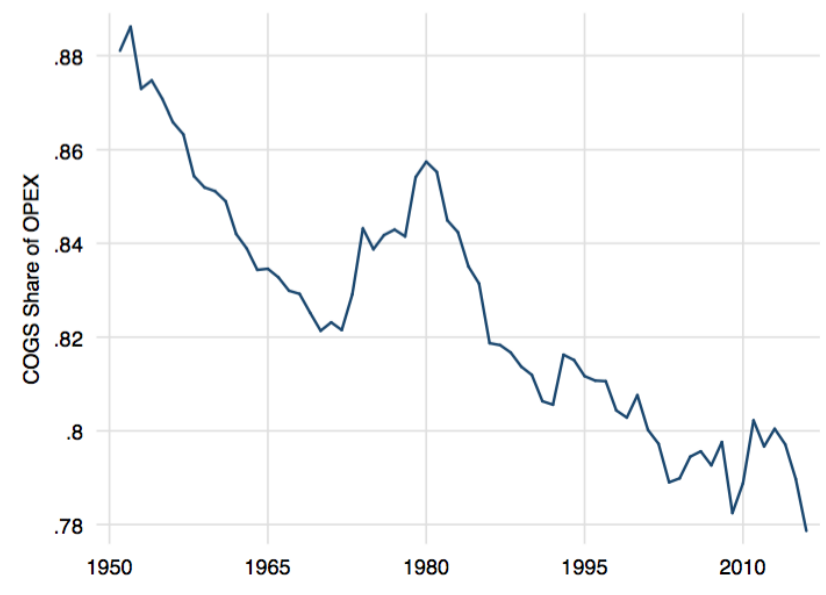
\includegraphics[width=0.48 \textwidth]{shareCOGS.PNG} & 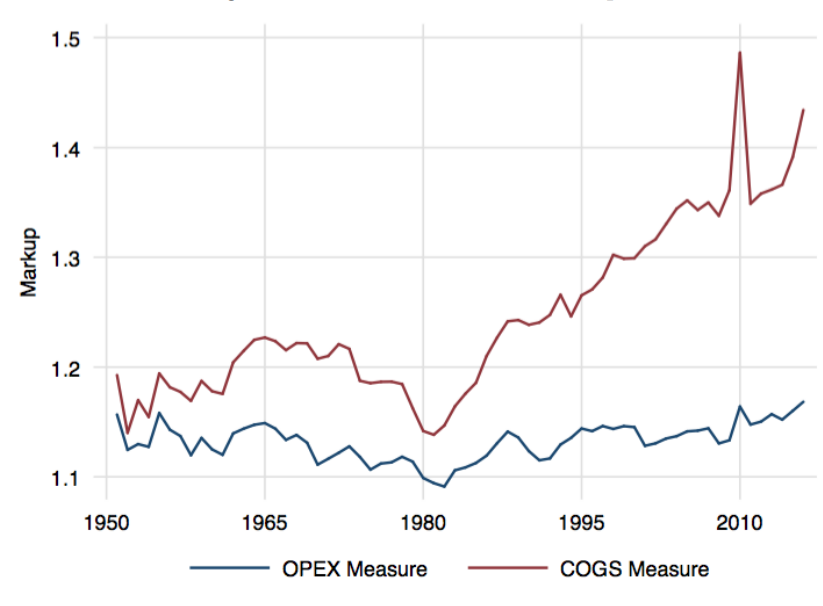
\includegraphics[width=0.48 \textwidth]{markups.PNG} \\ 
    \end{tabular}
\caption{Share of ``Cost of Goods Sold'' in total expenditures (left)  \& resulting markups (right) \\ figures 2 and 4 from  \cite{traina2018aggregate}}
\label{fig:traina}
\end{figure}

In a response to various comments raised by their initial work \citep{de2018some}, the authors defend their choice of COGS as a measure of variable input by arguing that SG\&A reflects fixed costs and thus does not adjust immediately. R\&D expenditure, marketing and advertising are long-term endeavour and they should not be used when calculating output elasticities or the ratio of variable costs to total sales. They argue that his measure of markups is not capturing markups but something closer to operation profit rate. According to them, this requires us to assume that overhead costs adjust flexibly and are perfect substitutes with traditional variable inputs in COGS. This assumption does not seem ill-founded to me. Increasing sales can be achieved through larger input quantities or more lreliable delivery, more aggressive marketing, etc. In particular, these inputs in the production process are more substitutable the large time horizon one considers.\\

\subsection*{Aggregation - Lack of differentiation in market analysis} Markets are heterogeneous in a number of dimensions and competition plays out differently in different markets. Some are subject to high entry costs (airlines), some have become less  competitive due to regulatory capture (broadband and communications), and some have been prone to collusion (chemicals). Concentration and market structure is an output of the competition process, and this process plays out very differently in different sectors. The IO literature has been sceptical of aggregating measures of market power across industries. The aggregation is a central tenet of the paper, but its legitimacy is questionable.\\

Importantly, this measure of markups lead to an unambiguous positive relationship between markups and firm size, across sectors.\\


\subsubsection{}

\section{Minor comments}

\section{Suggested extension}

\subsection*{Input-output linkages}

Important economic question, spurred by the rise of firm profit shares, in particular for large firms.\\

\subsection*{Linking higher markups to innovation rates} Higher fixed costs and higher markups mean that taking the incumbent's position as a market leader has become a more profitable goal. Given the richness of the \textit{Compustat} data, it is a shame that the authors did not relate their markup measure to innovation. two questions would be interesting to address: does innovation by incumbent decrease with higher markups? And does innovation by challenging firms increase? An effort in this direction is the works of \cite{aghion2008competition} and \cite{aghion2019theory} who find that there is an inverted U-shape relationship between productivity growth and markups.

\section*{Conclusion}

\subsection{The many causes of the rise of market power} Ultimately, this article is a somewhat convincing piece of evidence that market power is rising in the US economy. As this question is multifaceted and hard to assess, the evidence documented by De Loecker and co-authors needs to be considered along with other bits of evidence that market power is rising. This includes increased market concentration \citep{autor2017concentrating}, rising profits \citep{barkai2019declining}, decreased investment \citep{gutierrez2017investment}, and large decreased labour share in concentrated markets \cite{azar2017labor}.

Causes of rising markups: technology. For instance Amazon, incredibly productive, gets a large market share and then capture larger market share. ``Amazon paradox'', price is low but could be much lower. Market structure: options but all coming from the same producer.\\

Consequences: Decline in business dynamism. Wage stagnation (wage as a share of GDP). Aggregate decline in the labour share. Reallocation of sales from low markups firms to superstar high markups firms.\\

Cost-based method from Bob Hall (1988), less demanding on the data. \\

Distinction between markup and market power. Market power should also take into account fixed costs.\\

Fact 1: heterogeneity in markups. Median is fairly flat. But sales-weighted increase, and top tail is mostly responsible for it. Rise for a few firms, not for all firms.\\

Fact 2: reallocation. Markup weighted by sales, vs. total costs. Olley-Pakes decomposition for weight and. Total markup: change due to the distribution initially a third increases and then declines, so mostly due to the fact that more business going to high firms vs. low firms. Net entry. Driven by change in market share = superstar effect. \\

Idea for paper: show what is the impact of network formation on rise of markups, compare to superstar, net entry, etc...\\

Fact 3: change in technology. Overhead cost has gone up -> important to explaining the Amazon paradox. Amazon invests A LOT. Positive relationship between marups and fixed costs. Firms that invest heavily make excess profits.\\

Mention Basile Grassi.\\

Fact 4: issue about the magnitude of the increase. Bob Hall: lesser increase when computing increase at the sector level. But what matters is the micro data. Aggregation is important! Jensen's inequality. A lot of the heterogeneity is within sector. Profit rate does not increase much though (7pp vs 40pp). But need to account for the change in technology.\\

Publicly traded firms are 40\% of GDP.\\

Role of regulation?. Similar trend in publicly traded firms around the world. \\

\textbf{Model}. Builds on Atkinson-Burstein (2008). Technology here means change in fixed cost. Productivity shocks embody the ``Amazon effect''.\\

Note that increased markups have negative effects on welfare, but positive productivity effect, either positive of negative selection effect of selection. Endogeneous labour supply: negative effect. Households work less.\\

\textbf{Macroeconomic consequences}. Fact 1: decline in labour dynamism. Price reflect marginal cost in competitive market. In monopolistic market, less pass through from input and to consumer. In market with market power, firm adjust to productivity shock much less. Decline in labour dynamism, driven by rise in market power.\\

Fact 2: wage stagnation. Shift in labour demand, firm with high markups lowers quantity in labour demanded. Driven by equilibrium effect through fact that output market is non-competitive. No input market not being competitive! No monopsony!\\

Fact 3: decline in labour share. At firm level, important. Firms with higher markups should demand less, so produce less, at individual firm level. Can write labour share as elasticity of labour divided by ... Estimate that elasticity is fairly stable, but rise in markups, should decline demand in labour. regression of labour share on markups: negative. In aggregate, rise in markups lead to decrease in labour share.\\

Two thirds of rise in markups come from reallocation.\\





\textbf{References}. Notes on Jan De Loecker's website. Special issue of the JEP.\\


Debate about the measurement of 

\newpage

\bibliographystyle{ecta}
\bibliography{bibliography}

\newpage

\section*{Appendix}

\end{document}

%------------------------------------------------------------------------------
% End of journal.tex
%------------------------------------------------------------------------------
